\documentclass[journal,12pt,twocolumn]{IEEEtran}
\usepackage{amsmath,amsfonts,amssymb,float,amsthm,gvv,listings,enumitem,mathtools,setspace}
\usepackage{graphicx}
\bibliographystyle{IEEEtran}
\vspace{3cm}
\title{NCERT Discrete}
\author{Pragnidhved Reddy\\EE23BTECH11050}
\date{}
\parindent 0px
\begin{document}
\maketitle
\newpage
\bigskip
\textbf{Question 10.5.2.8:}\\
An AP consists of $50$ terms of which $3^{rd}$ term is $12$ and the last term is $106$. Find the $29^{th}$ term.\\
\solution 
\begin{table}[H]
\centering
\begin{tabular}{|c|c|c|}\hline
\textbf{Parameter} & \textbf{Value} & \textbf{description}\\ \hline
$x(2)$ & $12$ & Third term\\ \hline
$x(49)$ & $106$ & Last term\\ \hline
$x(0)$ & $$ & First term \\ \hline
$d$ & $$ & Common difference\\ \hline
$x(n)$ & $(x(0)+nd)u(n)$ & general term \\ \hline
\end{tabular}
\caption{Input parameters}
\label{tab:table1}
\end{table}
\begin{align}
\myvec{x(2) \\ x(49)}
&=
\myvec{1 & 2 \\ 1 & 49}
\myvec{x(0) \\ d}
\\[5pt]
\myvec{12 \\ 106}
&=
\myvec{x(0) + 2d \\ x(0) + 49d}
\\[5pt] 
&= \myvec{x(0)+2d &| 12 \\ x(0)+49d &| 106} \\
\quad R_2&\rightarrow R_2-R_1\\[5pt]
\label{eq:5}
&= \myvec{x(0)+2d &| 12 \\ 47d &| 94}
\end{align}
 From \eqref{eq:5}, we get
\begin{align}
\implies &x(0)=8\\
\implies &d=2
\end{align}
From the \tabref{tab:table1} :
\begin{align}
x(n)&=(x(0)+nd)u(n)\\
\implies x(n)&=(8+2n)u(n)
\end{align}
 Finding $x(28)$ :
\begin{align}
x(28)&=x(0)+28(2)\\
\implies x(28)&=64
\end{align}
 Z-transform :
\begin{align}
\implies &X(z)=\frac{8-6z^{-1}}{(1-z^{-1})^2} \quad \abs{z}>1
\end{align}\\[130pt]
\begin{figure}[h!]
    \centering
    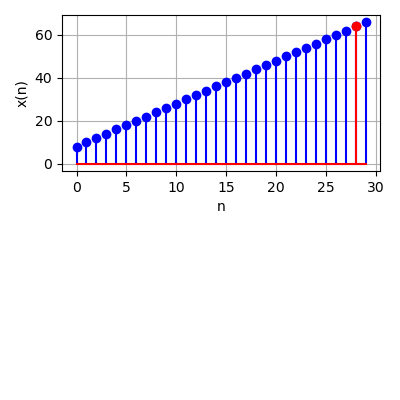
\includegraphics[width=\columnwidth]{figs/plot.png}
    \caption{graph of the given AP}
    \label{fig:1}
\end{figure}
\end{document}
